\documentclass{article}
\usepackage{graphicx}
\usepackage{listings}
\usepackage{xcolor}
\usepackage{hyperref}

\lstset{
	basicstyle=\ttfamily\small,
	keywordstyle=\color{blue},
	stringstyle=\color{red},
	commentstyle=\color{gray},
	showstringspaces=false,
	numbers=left,
	numberstyle=\tiny\color{gray},
	frame=single,
	breaklines=true,
	captionpos=b
}

\title{RPC File Transfer System}
\author{Le Anh Quang}
\date{}

\begin{document}
	
	\maketitle
	
	\section*{Design of the RPC Service}
	The RPC service is implemented using XML-RPC, a remote procedure call protocol that uses XML to encode calls and HTTP as a transport mechanism. The server provides three main functionalities:
	\begin{itemize}
		\item upload(fileName, content): Upload files to the server.
		\item download (fileName): Download files from the server.
		\item list(): List all files available on the server.
	\end{itemize}
	
	The system is designed with a server-client model:
	\begin{itemize}
		\item The server hosts the files and handles client requests.
		\item The client interacts with the server to perform file operations.
	\end{itemize}
	
	\begin{figure}
		\centering
		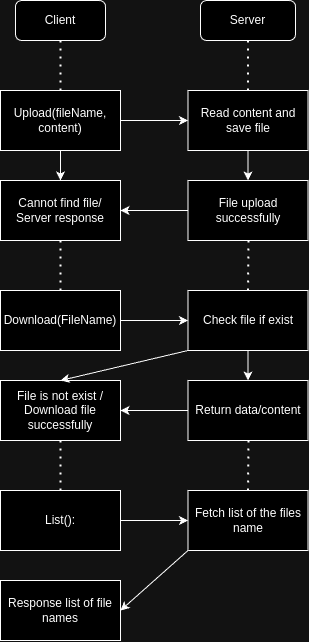
\includegraphics[width=0.8\textwidth]{RPC_design.png}
		\caption{High-Level Design of the RPC Service}
		\label{fig:rpc_design}
	\end{figure}
	
	\section*{System Organization}
	The server and client scripts are written in Python. 
	\begin{itemize}
		\item The server script (\texttt{server.py}) sets up the RPC server and registers functions for file operations.
		\item The client script (\texttt{client.py}) interacts with the server via an XML-RPC proxy.
	\end{itemize}
	
	\begin{figure}
		\centering
		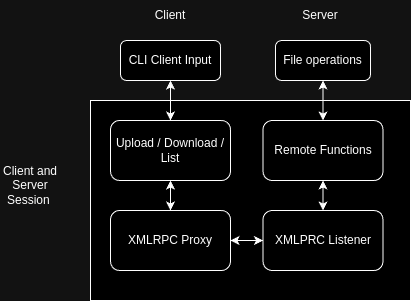
\includegraphics[width=0.8\textwidth]{System_Design.png}
		\caption{System Organization Diagram}
		\label{fig:system_organization}
	\end{figure}
	
	\section*{Implementation of the File Transfer}
	The following code snippets showcase the implementation of key functionalities:
	
	\subsection*{Client side:}
	\begin{lstlisting}[language=Python, caption={Client-side Upload Function}, label={lst:client_upload}]
import xmlrpc.client
import os
from typing import Dict, Callable


def upload(argument):
	server = argument[0]
	filename = argument[1]
	
	if not os.path.exists(filename):
		return "File does not exist"
	
	with open(filename, "rb") as file:
		content = file.read()
	
	response = server.upload(filename, content)
	
	return response


def download(argument):
	server = argument[0]
	filename = argument[1]
	content = server.download(filename)
	
	if not content:
		return "File not found"
	else:
		with open(filename, "wb") as f:
			f.write(content.data)
	return f"File {filename} downloaded successfully."


def list(argument):
	server = argument[0]
	files = server.list()
	return files


if __name__ == "__main__":
	host = ""
	port = 8080
	
	server = xmlrpc.client.ServerProxy(f"http://{host}:{port}/", allow_none=True)
	options = {
		"UPLOAD": upload,
		"DOWNLOAD": download,
		"LIST": list,
	}
	while True:
		try:
			userInput = (
			input("Enter operation (UPLOAD <file_name>, DOWNLOAD <file_name>, LIST) or QUIT to exit: ").strip()
			)
			userInput = userInput.split(" ")
			while userInput.count(" "): 
				userInput.remove(" ")
			operation = userInput[0].upper()
			argument = userInput[-1 : ]
			
			argument = [server] + argument
			
			if operation == "QUIT":
				break
			
			if operation not in options:
				print("Invalid operation")
				continue
			else:
				response = options[operation](argument)
				print("Response from server:", response)
			
		except Exception as e:
		print(f"Error: {e}")
		continue
	\end{lstlisting}
	
	\subsection*{Server Side:}
	\begin{lstlisting}[language=Python, caption={Server Main Function}, label={lst:server_main}]
import xmlrpc.server
import os

def download(fileName):
	if (os.path.exists(fileName)):
		with open(fileName, 'rb') as f:
			content = f.read()
		return content    
	else:
		return False

def upload(fileName : str, content : bytes):
	with open(fileName, "wb") as f:
		f.write(content.data)
	return "Successfully"

def list():
	fileList = os.listdir()
	return fileList

def main():
	host = "192.168.127.103"
	port = 8080
	server = xmlrpc.server.SimpleXMLRPCServer((host, port), allow_none=True)
	print("Start the server")
	server.register_function(upload, "upload")
	server.register_function(list, "list")
	server.register_function(download, "download")
	server.serve_forever()
	
	return 

if __name__ == "__main__":
	main()
	\end{lstlisting}
	
\end{document}
